\documentclass{article}
\usepackage{style}
\title{Quarterly Exam 1 (LoM DE Winter/Spring 2025)}
\author{Garud Shah}
\begin{document}
    \maketitle
    \newpage
    \begin{problem}[Problem 1]
        Consider 
        \begin{align}
            xy'-2y=0.
        \end{align}
        \begin{enumerate}[(a)]
            \item Find the general solution.
            \item Graph five solutions.
            \item What does the existence and uniqueness theorem have to say 
        \end{enumerate}
    \end{problem}
    \begin{solution}[Solution 1a]
        We add $2y$ to both sides to get:
        \begin{align}
            xy' = 2y.
        \end{align}
        As this is seperable, we perform the method for solving seperable equations. Thus:
        \begin{align}
            xy' &= 2y \\ 
            \dfrac{y'}{2y} &= \dfrac{1}{x} \\ 
            \int \dfrac{dy}{2y} &= \int \dfrac{dx}{x} \\ 
            \dfrac{1}{2} \log |y| &= \log |x| + C\\ 
            |y| &= A|x|^2, \text{ }A >0 \\ 
            y &= Ax^2, \text{ } A \ne 0 \\ 
            y &= Ax^2, \text{ } A \in \RR.
        \end{align}
        However when we removed the absolute value this gave us branches, thus the general solution is:
        \begin{align}
            y(x) =
            \begin{cases}
                A_1x^2, &y \ge 0 \\ 
                A_2x^2, &y < 0.            
            \end{cases},A_1, A_2 \in \RR
        \end{align}
        \begin{remark*}[Footnotes] \hfill 
            \begin{enumerate}
                \item Converting Eqn (1.1.2) to (1.1.3) drops the zero solution.
                \item (1.1.7) to (1.1.8) \textit{looks} like we added a solution out of nowhere, but we just added the solution we dropped in Footnote 1.1.1.
            \end{enumerate}
        \end{remark*}
    \end{solution}
    \newpage
    \begin{solution}[Solution 1b]
        \hfill \break
        \begin{center}
            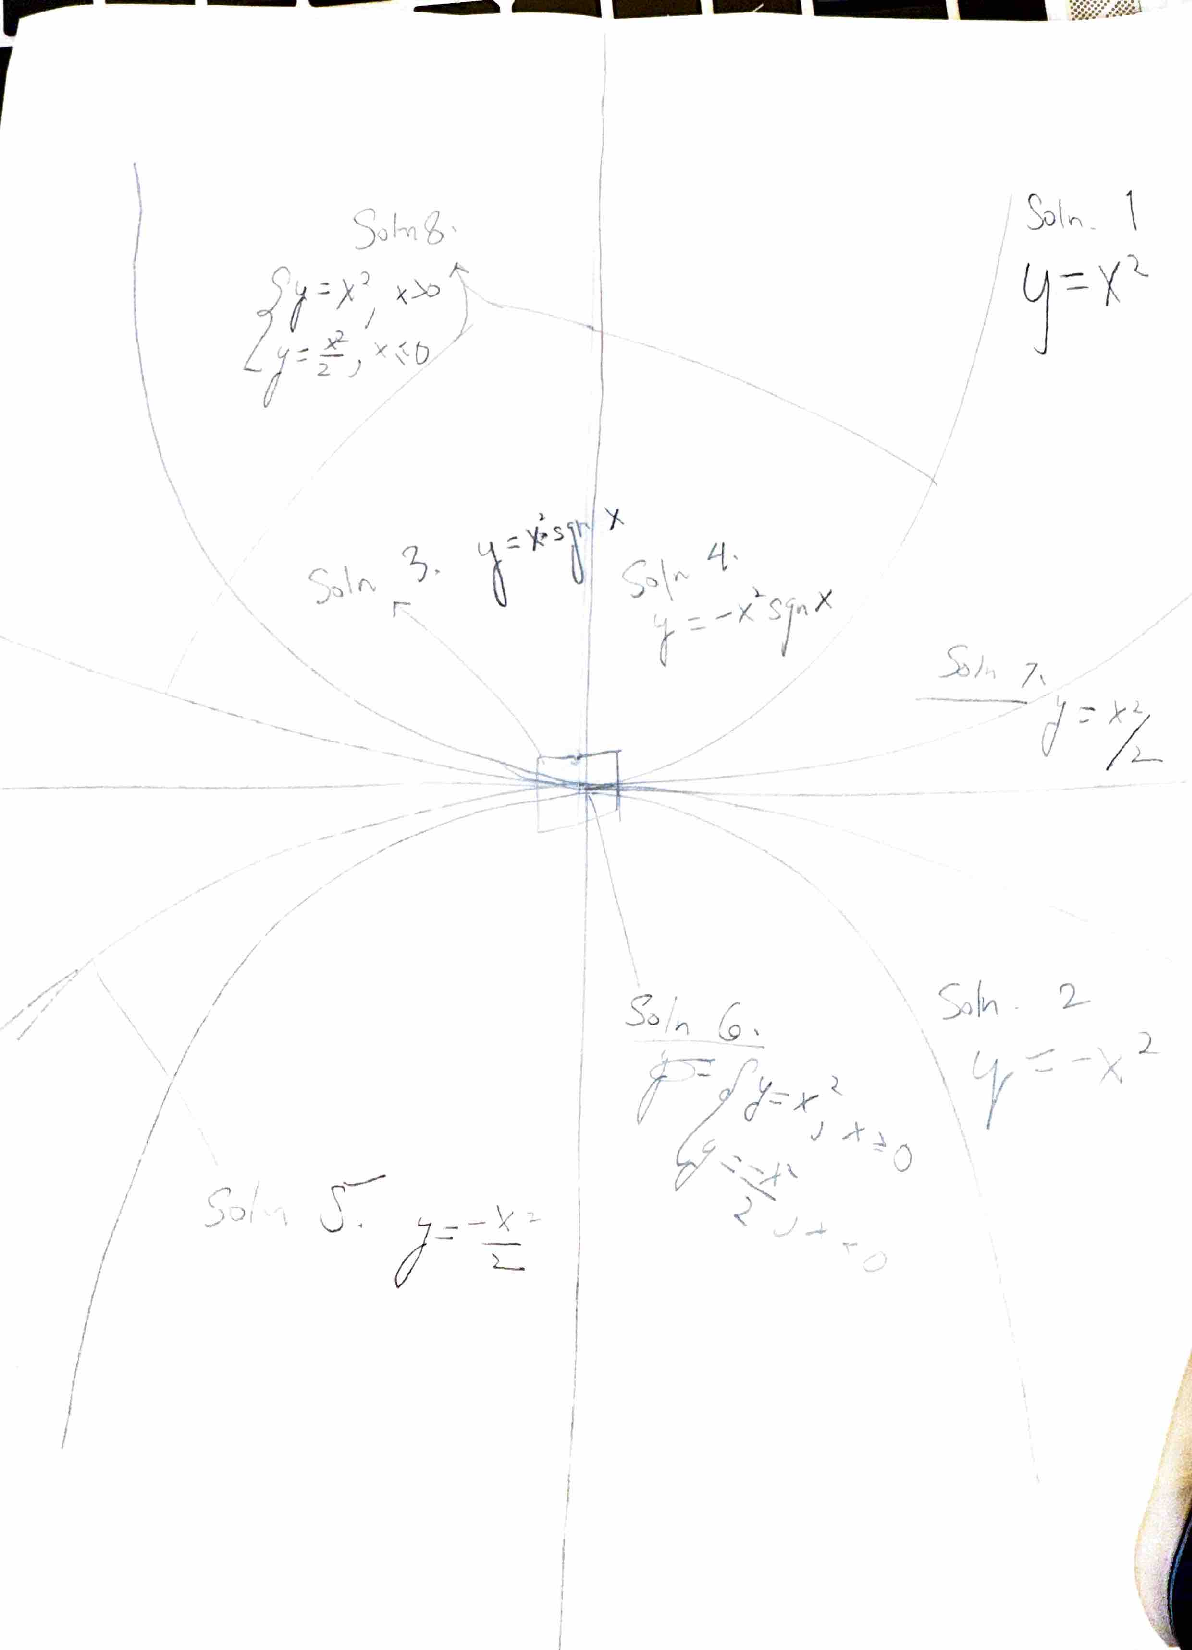
\includegraphics[scale=0.5]{images/1/B.pdf}
        \end{center}
        Extrapolating, there are infinitely many solutions through any point.
    \end{solution}
    \begin{solution}[Solution 1c]
        The existence and uniqueness theorem acts on:
        \begin{align*}
            xy' &= 2y \\ 
            y' &= \dfrac{2y}{x}.
        \end{align*}
        Thus we can use the existence and uniqueness theorem when $x \ne 0$. It does hold in this scneario in some local window, as all of our `distinct' solutions 
        are actually the same when we restrict to one side of the origin.
    \end{solution}
    \newpage
    \begin{problem}
        Consider the differential equation:
        \begin{align}
            y' = e^{y-x}.
        \end{align}
        \begin{enumerate}
            \item Sketch a direction field of the differential equation.
            \item Show that $y=x$ is a solution to the DE.
            \item What are the possible behavious of the solutions as $y \rightarrow \infty$?
        \end{enumerate}
    \end{problem}
    \begin{solution}[Solution 2a]
        \hfill \break
        \begin{center}
            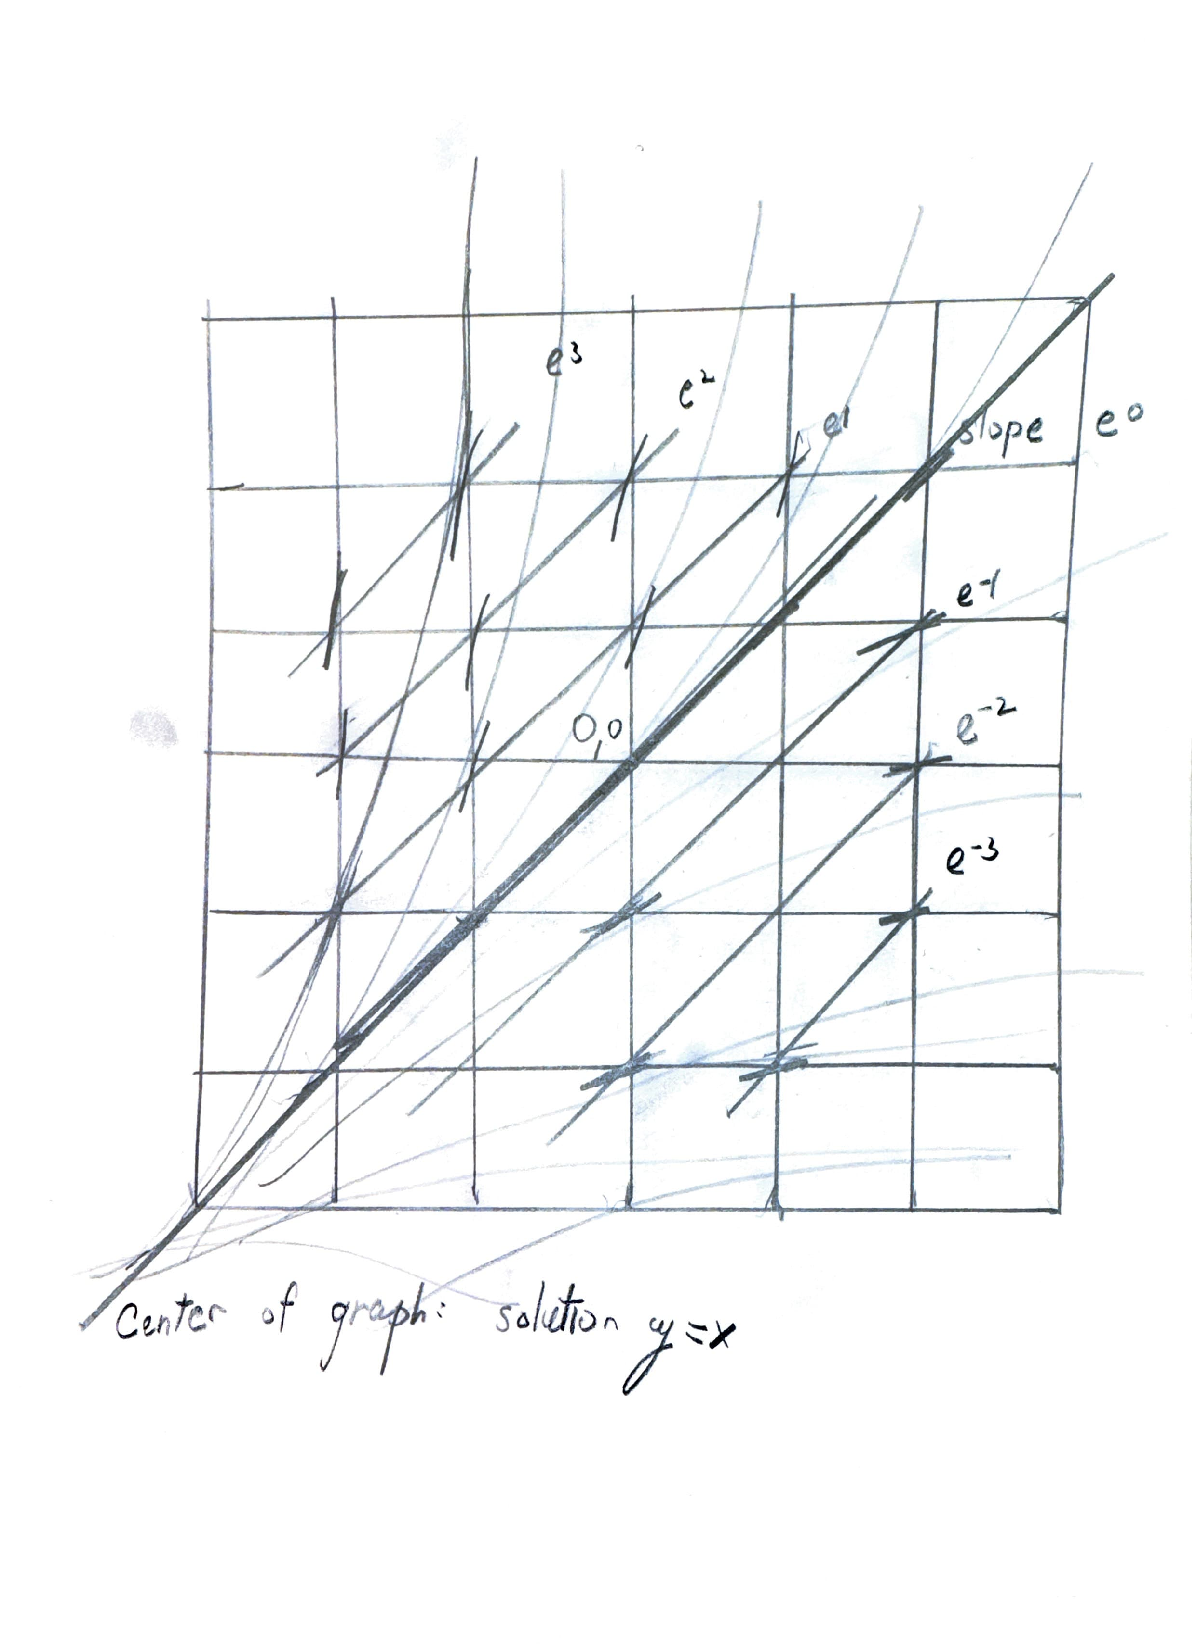
\includegraphics[scale=0.5]{images/2/A.pdf}
        \end{center}
    \end{solution}
    \newpage
    \begin{solution}[Solution 2b]
        Note that as $x=y$, $e^{y-x} = 1$ which is the slope everywhere.
    \end{solution}
    \begin{solution}[Solution 2c]
        Taking a look at the lightly drawn functions, they either:
        \begin{itemize}
            \item Going TO infinity they either
            \begin{itemize}
                \item increase super fast
                \item increase super slow
                \item stay as $y=x$
            \end{itemize}
            \item To negative infinity they have a asymptote of $y=x$ approacing negative infinity.
        \end{itemize} 
    \end{solution}
    \newpage 
    \begin{problem}[Problem 3, modified/generalized]
        Given the following differential equation:
        \begin{align}
            T' = k(T_0 - T),
        \end{align}
        find:
        \begin{enumerate}[(a)]
            \item the general solution.
            \item If $T(0) = T_i$, find when $T(t) = T_f$ if $T_i < T_f < T_0$ or $T_0 < T_f < T_i$.
        \end{enumerate}
    \end{problem}
    \begin{solution}[Solution 3a]
        Note that:
        \begin{align}
            T' &= k(T_0 - T) \\ 
            \dfrac{T'}{k(T_0 -T)} &= 1 \\
            \int \dfrac{dT}{k(T_0 - T)} &= \int dt \\ 
            -k \log |T-T_0| &= t + C\\ 
            T-T_0 &= Ae^{-t/k} \\
            T &= Ae^{-t/k} + T_0
        \end{align}
        (A similar note as Footnotes 1 can be made here with the lost and gained solution being $T \equiv T_0$).
    \end{solution}
    \begin{solution}[Solution 3b]
        We have:
        \begin{align}
            T_i &= Ae^{-0/k} + T_0 \\ 
            A &= T_i - T_0 \\ 
            T_f &= (T_i - T_0)e^{-t/k} + T_0 \\ 
            T_f - T_0 &= (T_i - T_0)e^{-t/k} \\ 
            e^{-t/k} &= \dfrac{T_f-T_0}{T_i - T_0} \\ 
            t &= k\log \left|\dfrac{T_i - T_0}{T_f - T_0}\right|.
        \end{align}
    \end{solution}
    \newpage
    \begin{problem}
        Solve the following differential equations:
        \begin{enumerate}[(a)]
            \item $(2x-y) dx  +(3y+x) dy =0 $
            \item $(3x^2 +y)dx + (x^2y - x) dy = 0$
            \item $(x+y+4) dx + (x-2y+3)dy = 0$
            \item $(x+y+4) dx + (2x + 2y +3) dy = 0$
        \end{enumerate}
    \end{problem}
    \begin{solution}[Solution 4a]
        This equation is HOMOGENOUS. Substitute $y = vx$, $\dfrac{dy}{dx} = v + v'x$:
        \begin{align}
            (2x-y) dx  +(3y+x) dy &=0 \\ 
            -\dfrac{2x-y}{3y+x} &= y' \\ 
            -\dfrac{2-v}{3v+1} -v&= v'x \\
            \dfrac{v'}{\dfrac{2-v}{3v-1} + v} &= -\dfrac{1}{x} \\ 
            \int \dfrac{dv}{\dfrac{2-v}{3v-1} + v} &= - \log x \\ 
            \int \dfrac{3v-1}{3v^2-2v+2} \, dv  &= - \log x \\  
            u = v - 1/3: \\ 
            \int \dfrac{u}{u^2 + \frac{1}{3}} \, du  &= - \log x  \\ 
            k = u\sqrt{3}: \\
            \int \dfrac{k}{k^2 + 1} \, dk  &= - \log x  \\ 
            \dfrac{1}{2} \log \left|k^2 + 1 \right| &= - \log |x| + C\\
            \dfrac{1}{2} \log \left|3\left(v-\dfrac{1}{3}\right)^2 + 1 \right| &= - \log |x| + C\\
            3\left(v-\dfrac{1}{3}\right)^2 - \left(\dfrac{C}{x}\right)^2 &= -1.
        \end{align}
    \end{solution}
    \newpage
    \begin{solution}[Solution 4b]
        Mutiply by an integrating factor $\mu(x,y)$ and get using test for exactness:
        \begin{align}
            \mu(x,y) + \mu_y(x,y)(3x^2+y) &= \mu_x(x,y)(x^2y-x) + (2xy -1) \mu(x,y),
        \end{align}
        so let $\mu$ be a function of $x$:
        \begin{align}
            \mu(x)(2-2xy) &= \mu'(x)'(x^2y-x) \\
            \mu &= \mu' \cdot x \cdot \dfrac{-1}{2} \\ 
            \dfrac{\mu'}{\mu} &= -\dfrac{2}{x} \\ 
            \log |\mu| &= -2\log|x| + C\\ 
            \mu = x^{-2}. 
        \end{align}
        Thus:
        \begin{align}
            \left(3+\dfrac{y}{x^2}\right)dx + \left(y-\dfrac{1}{x}\right)dy &= 0 \\
            F(x,y) = 3x - \dfrac{y}{x} + g(y) &= \dfrac{y^2}{2} - \dfrac{y}{x} + h(x) = 3x + \dfrac{y^2}{2} - \dfrac{y}{x} \\ 
            3x + \dfrac{y^2}{2} - \dfrac{y}{x} &= C. 
        \end{align}
    \end{solution}
    \newpage
    \begin{solution}[Solution 4c]
        This is an equation with linear coeffiecents. Let $y = y_0 - \dfrac{1}{3}$, $x = x_0 - \dfrac{11}{3}$. Then:
        \begin{align}
            (x_0 + y_0)dx + (x_0-2y_0)dy &= 0 \\ 
            y' &= -\dfrac{x_0 + y_0}{x_0 - 2y_0},
        \end{align}
        and now let $y_0 = x_0 v$:
        \begin{align}
            xv' + v &= -\dfrac{1+v}{1-2v} \\ 
            xv' &= - \left(\dfrac{1+2v^2}{1-2v} \right) \\ 
            \log x &= \int - \dfrac{1-2v}{1+2v^2} \, dv \\
            u &= \sqrt{2} v \\ 
            \int \dfrac{1-2v}{1+2v^2} \, dv &= \dfrac{1}{\sqrt{2}}\int- \dfrac{1}{1+u^2}\, du + \sqrt{2} \int \dfrac{u}{1+u^2} \, du \\ 
            \log x + C &= \dfrac{1}{2} \log |2v^2 + 1| - \sqrt{2} \arctan \left(\sqrt{2}v \right) \\ 
            C &= \dfrac{1}{2} \log (2y^2 + x^2) - 2 \log |x| - \sqrt{2}\arctan \left(\dfrac{3y + 1}{3x+11}\right).
        \end{align}
    \end{solution}
    \newpage
    \begin{solution}[Solution 4d]
        Note that:
        \begin{align}
            (x+y+4)dx + (2x+2y+3)dy &= 0 \\ 
            y' &= -\dfrac{2(x+y+2)-1}{x+y+1},
        \end{align}
        and letting $k = x+y+1$,
        \begin{align}
            k' &= 3 - \dfrac{1}[k] \\
            \int \dfrac{k}{3k-1} dk &= x \\ 
            \dfrac{1}{3} \int 1 + \dfrac{1}{k - 1/3} dk &= x \\ 
            k + \log |3k-1| - 3x &= C \\ 
            \log|3x+3y+2| + y-2x &= C. 
        \end{align}
    \end{solution}
    \newpage
    \begin{problem}[Problem 5, parts removed similar to AoPS]
        \hfill \break
        \begin{enumerate}[(a)]
            \item Show that if $y_1$ is a particular solution to the Ricatti Equation:
            \begin{align}
                y' = A(x)y^2 + B(x)y + C(x),
            \end{align}
            then the substitution $y = y_1 + \dfrac{1}{v}$ transforms our equation into 
            \begin{align}
                v' + (B(x) + 2A(x)y_1(x))v = -A(x).
            \end{align}
            \item Solve the Ricatti Equation:
            \begin{align}
                y' = y^2 + \dfrac{y}{x} - \dfrac{3}{x^2}.
            \end{align}
        \end{enumerate}
    \end{problem}
    \begin{solution}[Problem 5a]
        Plug in:
        \begin{align}
            y_1' - \dfrac{v'}{v^2} &= A(x)\left(\dfrac{1}{v} + y_1(x)\right)^2 + B(x)\left(\dfrac{1}{v} + y_1(x)\right) + C(x) \\ 
            -v' &= A(x) + 2vy_1(x)A(x) + B(x)v \\ 
            -A(x) &= v' + (B(x) + 2A(x)y_1(x))v
        \end{align}
    \end{solution}
    \newpage
    \begin{solution}[Problem 5b]
        Use the fact that $xy=1$, or $y_1 = \dfrac{1}{x}$ is a solution (as $y' = -\dfrac{1}{x^2}= RHS$)and use 5a:
        \begin{align}
            v' + (B(x) + 2A(x)y_1(x))v &= -A(x) \\ 
            v' + \dfrac{3v}{x} &= -1.
        \end{align}
        Multiply by a integrating factor $\mu(x)$:
        \begin{align}
            \mu'(x) = \dfrac{3}{x}\mu(x) \\
            \dfrac{\mu'}{\mu} = \dfrac{3}{x} \\ 
            \mu = x^3.
        \end{align}
        Then:
        \begin{align}
            (x^3v)' &= -x^3 \\ 
            vx^3 &= -\dfrac{x^4}{4} + C \\
            v &= -\dfrac{x}{4} + \dfrac{C}{x^3}.
        \end{align}
        Thus:
        \begin{align}
            y(x) = \dfrac{1}{x} + \dfrac{4x^3}{Cx-x^4}.
        \end{align}
    \end{solution}
    \newpage
    \begin{problem}[Problem 6, modified, EXTRA CREDIT]
        Consider the Bernoulli Equation:
        \begin{align}
            y' + \left(- \dfrac{2}{x}\right) y &= -\dfrac{y^3}{x^3}. 
        \end{align}
        (including the solution $y=0$)
        \begin{enumerate}[(a)]
            \item Find the general solution.
            \item For the solutions $\dfrac{x^4}{y^2} - x^2 = C$, when does the implicit function theorem guarentee a unique explicit solution?
            \item Are there any points with more than one explicit solution, and with none at all?
            \item What does existence and uniqueness say about this?
        \end{enumerate}
    \end{problem}
    \begin{solution}[Solution 6a]
        We divide through by $y^3$:
        \begin{align}
            \dfrac{y'}{y^3} + \left(- \dfrac{2}{x}\right) y^{-2} &= \dfrac{-1}{x^3}. 
        \end{align}
        Now substitute $y_1 = y^{-2}$. Then:
        \begin{align}
            \dfrac{-y_1'}{2}+ \left(- \dfrac{2}{x}\right) y_1 &= \dfrac{-1}{x^3} \\ 
            y_1' + \left(\dfrac{4}{x}\right) y_1 &= \dfrac{2}{x^3}.
        \end{align}
        This is a linear. Use the integrating factor $x^4$ to get:
        \begin{align}
            (y_1 x^4)' &=2x \\ 
            \dfrac{x^4}{y^2} &= x^2 + C. 
        \end{align}
    \end{solution}
    \begin{solution}[Solution 6b]
        Note that we need the function to be well-defined - or $y \ne 0$ - and it to have a partial derivative (same condition!) \\~\\
        Thus the points are those with $y \ne 0$.
    \end{solution}
    \begin{solution}[Solution 6c]
        Not with none if $x \ne 0$: the explicit solutions $\pm \sqrt{\dfrac{x^4}{x^2 + C}}$ exist for all points $y\ne 0$ BUT we can mix and match at $(x,y) =0$ thus every 
        point has infinitely many solutions through it (unless $x = \pm y$!). But when $x =0$, either $y=0$ or nothing.
    \end{solution}
    \begin{solution}[Solution 6d]
        E and U theorem works when $x \ne 0$, but it provides only \textit{local} information which is compatible with our knowledge.
    \end{solution}
    That's it! This took me almost four hours to write up, mainly because I can't remember integrals that I probably \textit{should} remember. 
    \begin{center}
        
\includegraphics{images/time.png}
    \end{center}
    (This is my timer...)
\end{document}